\section{Introduction}
\label{sec:intro}

\begin{figure*}[t]
  \centering
  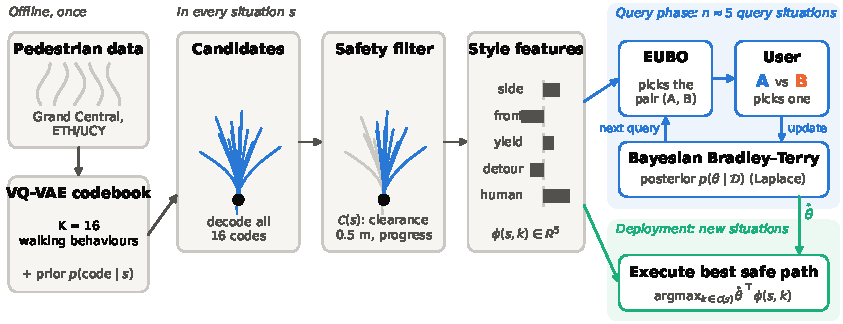
\includegraphics[width=\linewidth]{figures/fig_architecture.pdf}
  \caption{Framework. Offline, a VQ-VAE learns a codebook of $K=16$ walking behaviours and a prior network from pedestrian
  trajectories. In every situation the codebook is decoded into candidate paths, unsafe ones are removed, and each safe candidate is
  described by five style features. In a few query situations EUBO picks a pair of safe candidates, the user answers which they prefer,
  and a Bayesian Bradley--Terry posterior over the preference is updated. In new situations, without further questions, the robot
  executes the safe candidate that is best under the posterior mean $\hat\theta$. Fig.~\ref{fig:overview} shows the steps on a real
  situation. Generated by \texttt{utils/figure\_architecture.py}.}
  \label{fig:architecture}
\end{figure*}

Robots increasingly share sidewalks, stations and shopping streets with people, and how such a robot moves through a crowd matters to
the person it serves -- the user who sends a delivery robot, rides in a wheelchair or walks alongside a guide robot. ``Socially compliant''
navigation, however, is not a single behaviour. Facing an oncoming pedestrian, one user wants the robot to slow down and let them pass,
another wants it to keep pace; one prefers it to pass behind people, another in front; one tolerates a wide detour around a group, another
wants the shortest safe path. People themselves differ in how close they pass others and how readily they give way
\citep{hall1966hidden}, so a single notion of good crowd behaviour leaves many users
dissatisfied.

Crowd-navigation methods nonetheless optimize one fixed objective. Model-based planners encode hand-tuned social costs, reinforcement-learning
policies maximize a designed reward, and imitation or generative planners reproduce the average pedestrian of their training data
\citep{helbing1995social,vandenberg2011reciprocal,chen2019crowd,kretzschmar2016socially,mavrogiannis2023core}. Adapting any of them to an individual requires retuning or
retraining. Preference-based learning offers a direct route: instead of specifying a reward, the user compares two behaviours and the robot
infers what they want~\citep{christiano2017deep,sadigh2017active}. In robotics, however, each comparison costs the user time and attention,
so a preference must be identified from a handful of answers, and the trajectories being compared must be meaningful to a person: safe,
plausible, and different in ways the user cares about.

Our key idea is to separate \emph{what} the robot can do from \emph{which} of those behaviours a particular user wants (Fig.~\ref{fig:architecture}).
For the first, we learn a discrete codebook of human walking behaviours with a VQ-VAE~\citep{vandenoord2017neural} trained on pedestrian
trajectories. Decoding the codebook in a given situation yields a small set of candidate paths that are human-like by construction and
differ in style -- passing left or right, ahead or behind, slowing down or keeping pace -- and a safety filter removes the ones that come too
close to anyone. For the second, we describe each safe candidate by five interpretable style features and model the user's preference as a
linear utility over them, learned with a Bayesian Bradley--Terry model~\citep{bradley1952rank} from A/B answers. Because the robot only
executes one path per situation after querying, the relevant objective is simple regret, and we choose each question by the expected utility
of the best option (EUBO)~\citep{astudillo2023qeubo}, which is one-step Bayes-optimal for it.

The data prior alone does not capture individual preferences: on held-out situations from Grand Central and ETH/UCY, always taking the most
human-like safe path leaves a normalized simple regret of 0.45--0.47 for simulated users, close to a random safe path (0.49). Five EUBO
queries reduce it to 0.09--0.12, with lower regret than random questions in all four settings and than an active-query baseline in three,
and as low as an information-gain query; the advantage over random questions holds for noisy, inconsistent and nonlinear simulated users.
The comparison with Direct Preference Optimization~\citep{rafailov2023direct}, the estimator behind much of current preference fine-tuning,
shows where the gain comes from: given the same questions, DPO and the Bradley--Terry posterior perform alike, but DPO has no posterior with
which to choose its questions. The candidate set matters as well: on shared Grand Central scenes, the candidates of a flow-matching
crowd-navigation planner~\citep{singha2026crowdfm} cover a much narrower range of behaviours than the codebook, which bounds what any learned preference
can achieve (union regret 0.35 vs 0.11 after five queries). Finally, in a closed-loop replay, following the learned preference keeps the
user's step regret at 0.10--0.14 without a significant change in collision rate.

\paragraph{Contributions.}
\begin{itemize}
  \item A walking-behaviour codebook learned with a VQ-VAE from pedestrian trajectories, which turns a situation into a small set of
        diverse, human-like candidate paths that a safety filter can check (Sec.~\ref{sec:candidates}).
  \item A linear preference over five interpretable style features, learned with a Bayesian Bradley--Terry model from A/B answers,
        with questions chosen by EUBO to minimize simple regret (Sec.~\ref{sec:preference}).
  \item A simple-regret evaluation protocol on held-out situations (Sec.~\ref{sec:regret}) and experiments on Grand Central and
        ETH/UCY that compare query selection (including information gain and users outside the model), a DPO estimator, a flow-matching candidate generator, and closed-loop execution
        (Sec.~\ref{sec:experiments}).
\end{itemize}
